%%% Theory %%%
\section{MARCOS WORKS IS THISSSSS!!}
\chapter{Theory(Simon)}
\section{The digital Image}
Working around digital images on computers is something that most can relate to, but there is a lot more to it than one realizes. Figure \eqref{fig:ip_ColoredToGrayscaleToBinary} shows what this chapter is all about; working with color, grayscale or binary images and the different attributes of each type.

\begin{figure}[htbp]
\centering
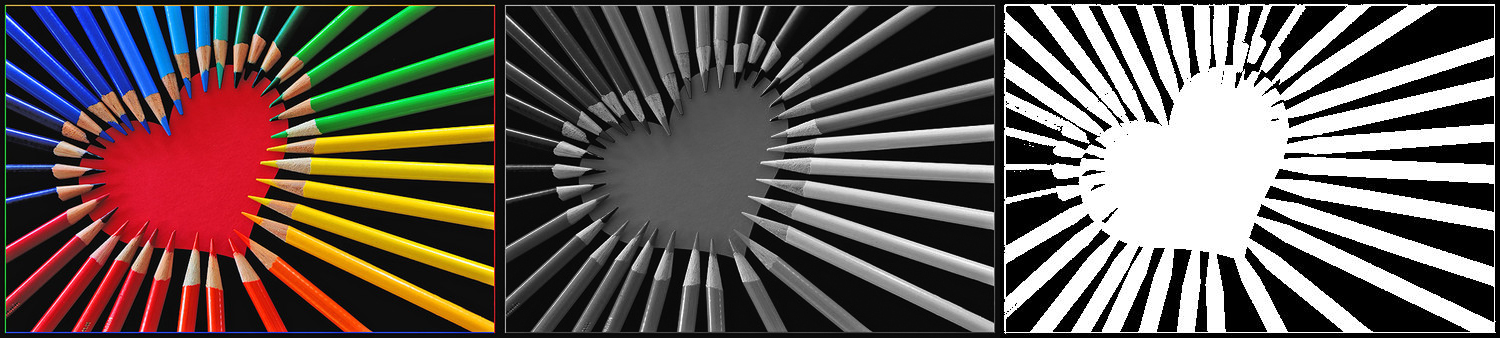
\includegraphics[width=1.00\textwidth]{Pictures/Theory/ColoredToGrayscaleToBinary.jpg}
\caption{Image illustrating a conversion from a colored image to grayscale and finally to binary}
\label{fig:ip_ColoredToGrayscaleToBinary}
\end{figure}

\subsection{8 bit Image and Grayscale Images}
In an 8 bit image, the 8 bit bit prefix describes the \textit{bit depth} of the image. The bit depth tells you about the amount of information you can store in a single pixel.
\\
An image with a single channel of information for each pixel in the x and y axis is typically a grayscale image, since each pixel is limited to information about a single hue. The information stored in each pixel is the intensity of the particular pixel. 8 bits evaluates to $2^8$ different states, meaning that a single 8 bit pixel can display 256 different levels of intensity. In addition one should note that logically the values of the pixels should be 1-256, but the fact is that a computer counts 0 as the first value and therefore the pixel value varies from 0-255, see figure \eqref{fig:ip_grayscale}. An 8-bit image is a widely spread format for an image, but it is however possible to create images with more depth and with more information for each individual pixel in the image. Examples of that are 16, and 32 bit images. A 16 bit depth is equal to $2^{16}$ different states, which means that each pixel can hold any one of 65,536 different shades of gray. Simultaneously a 32 bit depth is equal to $2^{32}$, which gives 4,294,967,296 different shades of gray. It should however be notified that working with 8 bit picture is the most standard format when doing computer operations, as it consumes less processing power than a similar looking 16- or 32 bit image.
\\
%As the human eye is not able to distinguish the huge numbers of photos hitting the eye, one have decided to quantify the number of photos hitting a cell. This is often quantified as bytes (8 bits), which applies to the binary system and also the structure of memory within a computer.
\\
%An image with one channel of information for each pixel in the x and y axis is called grayscale image, which describes the intensity of light in that specific pixel. The value of the pixel applies to the binary system with the value of $2^8$ when working with 8 bit pictures, which is 256. That means by having an 8-bit picture with 256 levels of intensity, it is possible for the computer to distinguish 256 different levels of one particular color, giving more depth. In addition one would note that the values of the pixels should be 1-256, but fact is that a computer counts 0 as the first value and therefore it is from 0-255. An 8-bit picture is a pretty standard format for a picture, but it is however possible to create images with more depth and with more information for each individual pixel in the picture.
\begin{figure}[htbp]
\centering
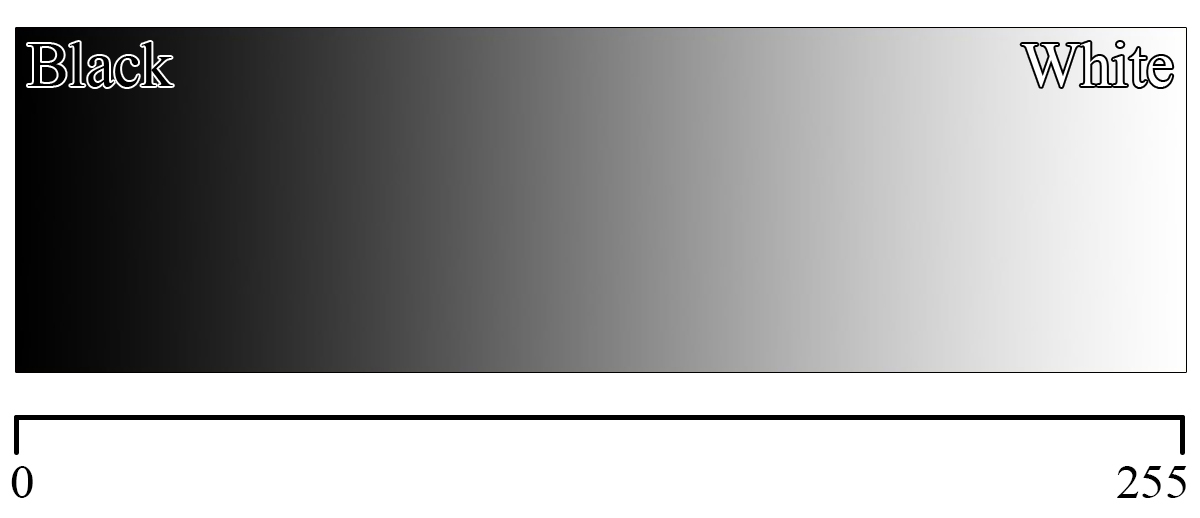
\includegraphics[width=1.00\textwidth]{Pictures/Theory/Grayscale.jpg}
\caption{Image illustrating the 256 different gradients of an 8 bit picture.}
\label{fig:ip_grayscale}
\end{figure}
 Illustrates 256 different levels of grayscale.\\

 
\subsection{Indexing an image}
When working with images on a computer and performing image processing, one often has to look at the individual pixels within an image to perform mathematical operations. Accessing specific pixels is however relatively easy as it's indexed cleverly.\\
Working around the pixels in a image is like working with a coordinate system. However instead of starting at the lower left corner, a picture is indexed from the upper left corner, starting in the point (0,0). Moving horizontally applies to the x-axis and moving vertically applies to the y-axis.\fixme{Did we mention openCV before? Maybe write something about how OpenCV stores images} In OpenCV pictures are stored in a matrix. The size of the matrix holding the pixel values of the x- and y-axis is as wide as the proportions of the image i.e. an image with a resolution of \textit{1024*1024} pixels is loaded, the highest coordinate assigned to pixels in the the matrix is (1023,1023). Figure \eqref{fig:ip_IndexingAPicture} Illustrates the theory of indexing a image in the y- and x-axis.\\
\begin{figure}[htbp]
\centering
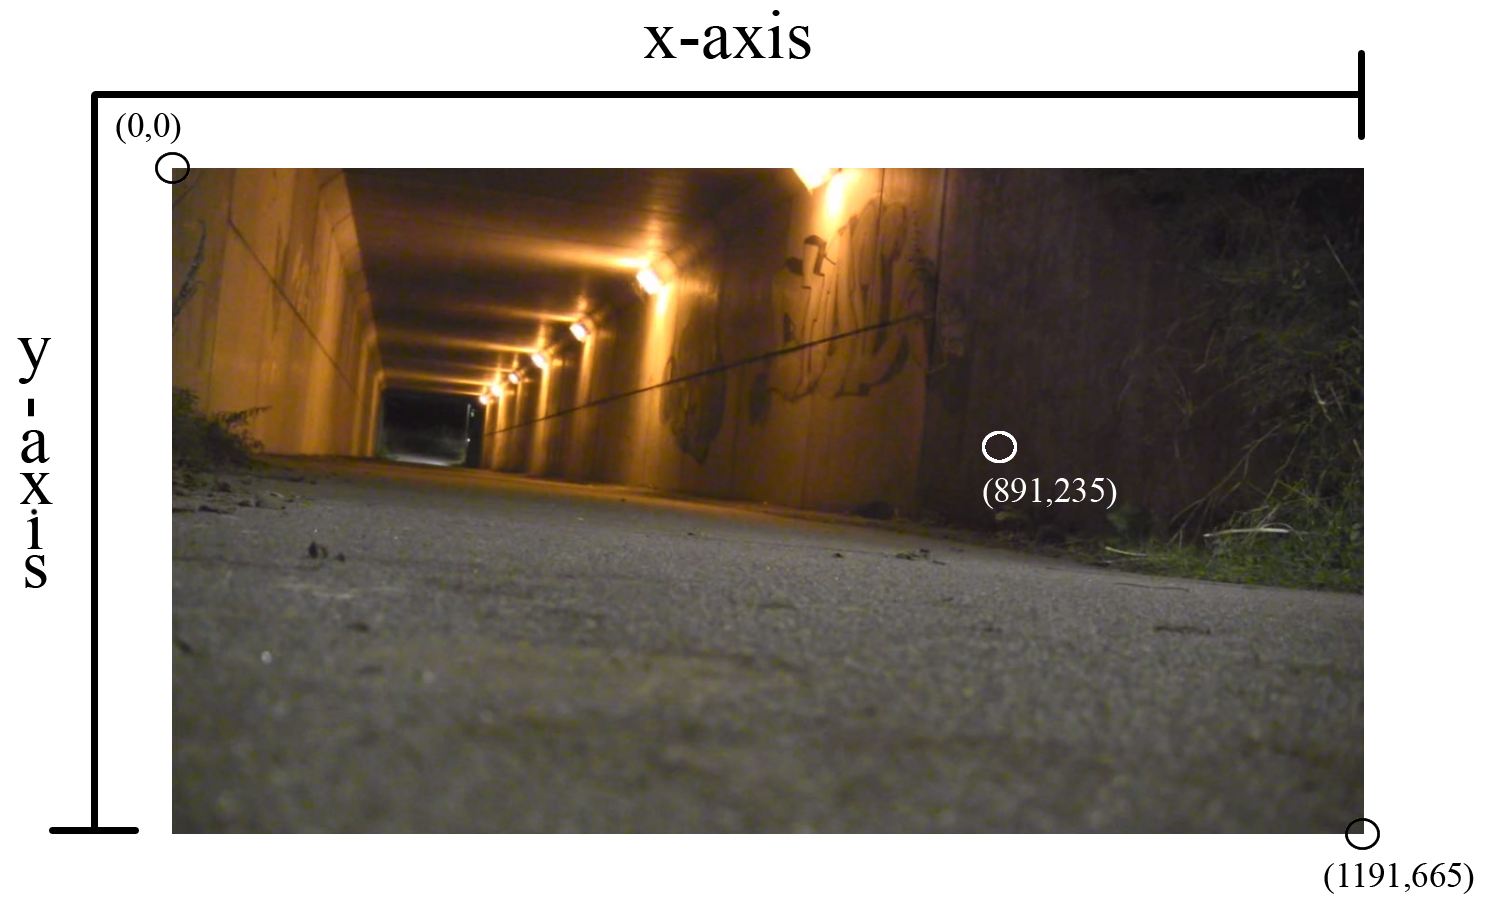
\includegraphics[width=1.00\textwidth]{Pictures/Theory/IndexingAPicture.png}
\caption{Image illustrating the principle of indexing a picture in x- and y-axis.}
\label{fig:ip_IndexingAPicture}
\end{figure}
  

\subsection{Working with Colored Images (RGB)}
Now that a basic knowledge regarding images has been established, the next leap into using images in calculations is to understand the basics of a color image.\\
Figure \eqref{fig:ip_ColorWheel} Illustrates the making of colors in relation to the RGB system.\\
\begin{figure}[htbp]
\centering
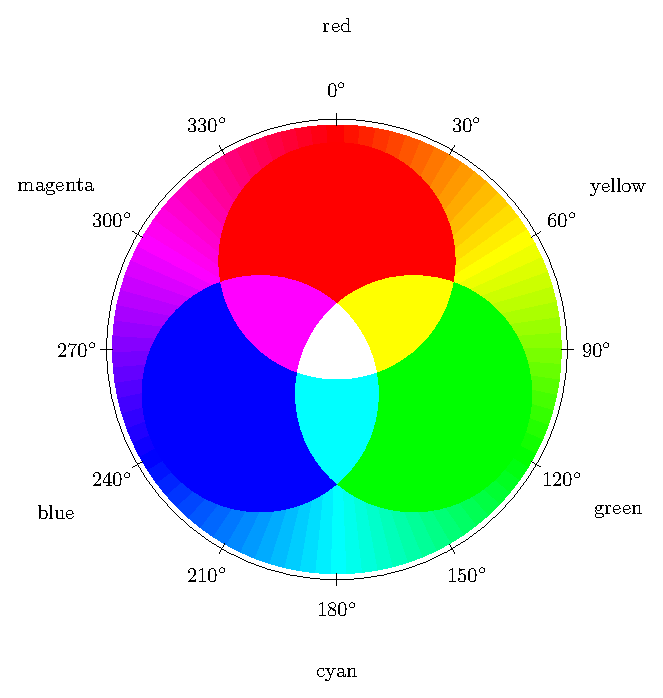
\includegraphics[width=0.70\textwidth]{Pictures/Theory/RGBColor.pdf}
\caption{Image illustrating the making of colors from http://www.texample.net/tikz/examples/rgb-color-mixing/}
\label{fig:ip_ColorWheel}
\end{figure}\\
\fixme{THIS IS WHERE I GOT TO -Marco}
Different from a grayscale image, a colored image consists of 3 channels of colors that each describe the value of the color in relation to red, blue or green, which are the primary colors from which all other colors are derived. The most significant different between grayscale images and colored images, is that now one would not describe the intensity of one specific color, but a mix of the red, green and blue color. In addition giving the red, green and blue pixel a value of 255 will produce white, while giving them all the value 0 would produce black, just as when working with grayscale images.\\
Knowing the specific values of the red, green and blue channels within an image gives the user a great advantage, especially when performing image manipulations in programming. If one wants to exclude a specific color in a mathematical operation, such as deriving colors adjoining to red from the input, one would simply have to create a threshold to segment the the minimum and maximum values of the red channel. The outcome should be a picture with a limited/controlled amount of red. 

\subsection{Binary Images}
One edge of image operations is binary pictures. In comparison to above-mentioned that is all about picture depth and pixel information, binary pictures is represented by two colors only in form of black and white. Using this indicates the use of a threshold, described in section \ref{sec:Thresholding}.\\
Using the tool correctly, one will be able to adjust the input so that only usable pixel information remains in the picture. However one should be careful when using thresholding, as it's easy to over- and undersegmentate an input.\\
Binary pictures are less resource demanding when performing mathematical operations as only two colors remain of the original input. In 


